\documentclass{beamer}
\usetheme{CambridgeUS}
\usepackage{enumerate}
\usepackage{amsmath,amsfonts,amssymb}
\usepackage{setspace}
%\usepackage{gensymb}
\usepackage{subfig}
\usepackage{float}
\usepackage{cellspace}
\usepackage{longtable}
\usepackage{hhline}
\def\inputGnumericTable{}
\usepackage{bigstrut}
\newcounter{saveenumerate}
\newcommand{\saveenumerate}{\setcounter{saveenumerate}{\value{enumi}}}
\newcommand{\restartenumerate}{\setcounter{enumi}{\value{saveenumerate}}}
\setlength{\abovedisplayskip}{0in}
\title{Assignment 7} 
\author[CS21BTECH11021]{Harshit Pant\\CS21BTECH11021}
\date{}
\providecommand{\pr}[1]{\ensuremath{\Pr\left(#1\right)}}
%\logo{\large \LaTeX{}}
\begin{document}
\begin{frame}
\titlepage
\end{frame}
\begin{frame}{Question}
\begin{block}{\textbf{Example 5.2 [Papoulis]}}
Let $X$ and $Y$ be two continuous random variables such that $Y=y$ and $X=x$ where $x,y\in\mathbb{R}$ with x and y related by the expression $y=x^2$. Find $\mathbf{F_Y(y)}$ and $\mathbf{f_Y(y)}$
\end{block}
\end{frame}
\begin{frame}{Solution}
\begin{block}{Definition/Properties}
\begin{align}
F_Y(y)&=\pr{Y\leq y}\\
\pr{a\leq x\leq b}&=F_X(b)-F_X(a)\\
f_Y(y)&=\dfrac{dF_Y(y)}{dy}
\end{align}
\end{block}
\begin{block}{}
If $y\geq 0$,
\begin{align}
&x^2\leq y\\
-\sqrt{y}\leq&\,x\leq \sqrt{y}\\
F_Y(y)&=\pr{-\sqrt{y}\leq x\leq \sqrt{y}}\\
F_Y(y)&=F_X(\sqrt{y})-F_Y(-\sqrt{y})
\end{align}
\end{block}
\end{frame}
\begin{frame}
\begin{block}{}
If $y<0$,\\x has no real values satisfying the inequality $x^2<y$
\begingroup
\addtolength{\jot}{.1in} 
\begin{align}
F_Y(y)&=\pr{\phi}\\
F_Y(y)&=0
\end{align}
\endgroup
\end{block}
\begin{exampleblock}{CDF}
\begingroup
\addtolength{\jot}{.1in}
\begin{align}
F_Y(y)&=\begin{cases}
				  F_X(\sqrt{y})-F_X(-\sqrt{y})&y\geq0\\
				  0&y<0\\
				  \end{cases}
\end{align}
\endgroup
\end{exampleblock}
\end{frame}
\begin{frame}
\begin{block}{PDF}
\begingroup
\addtolength{\jot}{.1in}
\begin{align}
f_Y(y)&=\begin{cases}
				 \dfrac{1}{2\sqrt{y}}(f_X(\sqrt{y})+f_X(-\sqrt{y}))&y>0\\
				 0&y\leq0
				 \end{cases}
\end{align}
\endgroup
\end{block}
\begin{exampleblock}{Case: $f_X(x)$ is even}
Let
\begingroup
\addtolength{\jot}{.1in}
\begin{align}
U(y)&=\begin{cases}
			  1&y>0\\
			  0&y\leq0
			  \end{cases}\\
f_Y(y)&=\dfrac{1}{\sqrt{y}}f_X(\sqrt{y})U(y)
\end{align}
\endgroup
\end{exampleblock}
\end{frame}
\begin{frame}
\begin{block}{Case (a): Gaussian Distribution}
Let $X$ be normally distributed with $\mu=0$ and $\sigma^2=1$.\\
$X\sim N(0,1)$
\begingroup
\addtolength{\jot}{.1in}
\begin{align}
f_X(x)&=\dfrac{1}{\sqrt{2\pi}}e^{-x^2/2}\\
f_Y(y)&=\dfrac{1}{\sqrt{2\pi y}}e^{-y/2}U(y)
\end{align}
\endgroup
\end{block}
\end{frame}
\begin{frame}
\begin{figure}[!tbp]
  \centering
  \subfloat[Gaussian/Normal Distribution.]{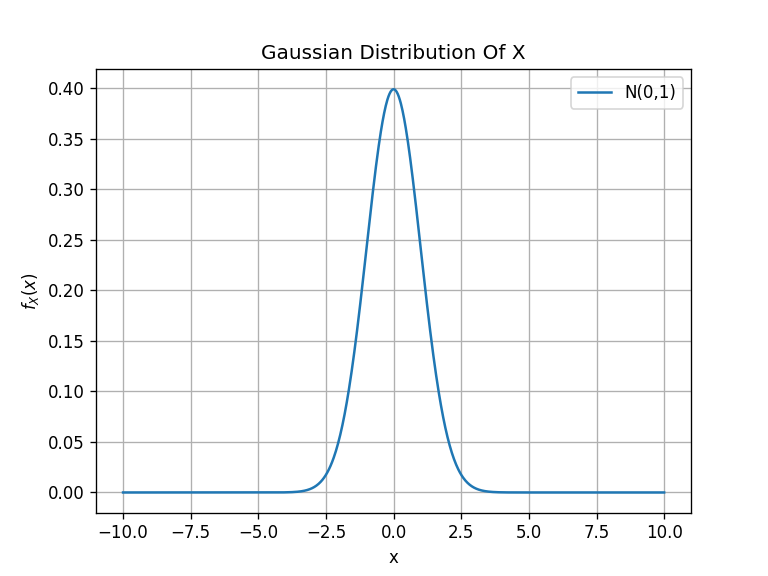
\includegraphics[width=0.5\textwidth]{1.png}\label{fig:f1}}
  \hfill
  \subfloat[PDF of Y.]{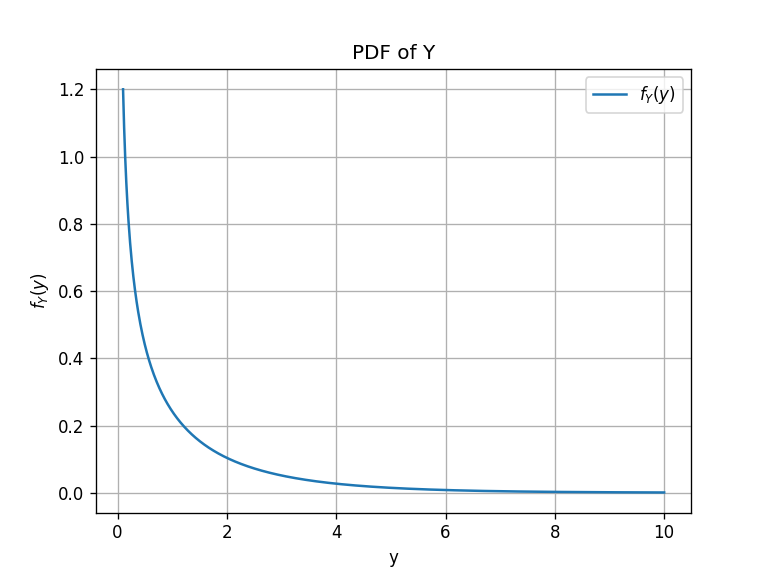
\includegraphics[width=0.5\textwidth]{2.png}\label{fig:f2}}
\end{figure}
\end{frame}

\begin{frame}
\begin{block}{}
On comparing, we notice that this represents a chi-square random variable with $n=1$
\end{block}
\begin{exampleblock}{Chi-sqaured Distribution}
\begin{align}
f_X(x,n)&=\begin{cases}
					\dfrac{1}{2^{n/2}\Gamma(n/2)}x^{n/2-1}e^{-x/2}&x>0\\
					0&x\leq0
					\end{cases}
\end{align}
\end{exampleblock}
\end{frame}
\begin{frame}
\begin{figure}[!tbp]
  \centering
  \subfloat[PDF for Chi-squared distribution.]{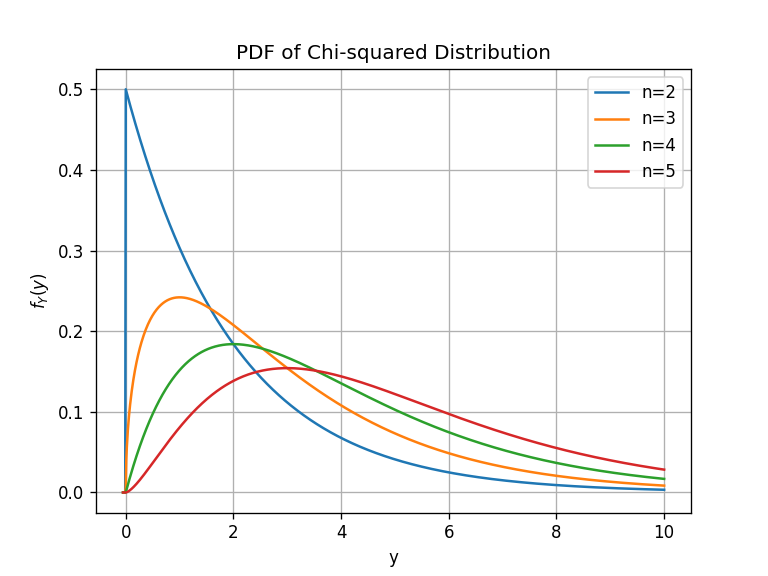
\includegraphics[width=0.5\textwidth]{6.png}\label{fig:f3}}
  \hfill
  \subfloat[Simulated CDF.]{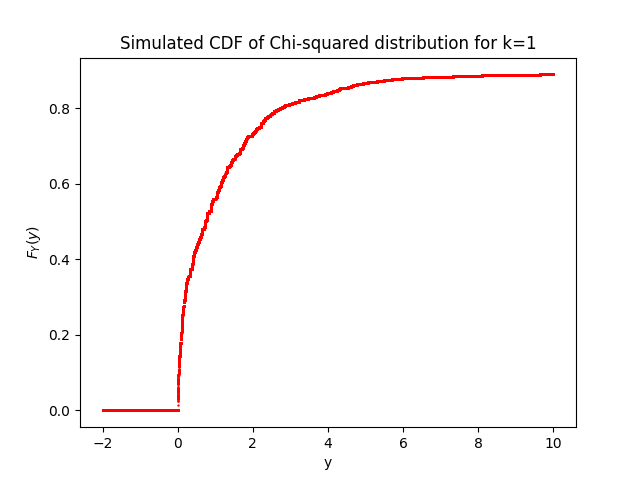
\includegraphics[width=0.5\textwidth]{fig1.png}\label{fig:f7}}
  \caption{Chi-squared distribution}
\end{figure}
\end{frame}
\begin{frame}
\begin{block}{Case (b): Uniform Distribution}
Let X be uniformly distributed in the interval $x\in(-1,1)$\\
\begingroup
\addtolength{\jot}{.1in}
\begin{align}
f_X(x)&=\begin{cases}
				 1/2&|x|\leq1\\
				 0&|x|>1
				 \end{cases}\\
f_Y(y)&=\begin{cases}
				 \dfrac{1}{2\sqrt{y}}&y\in(0,1]\\
				 0&y\notin(0,1]
				 \end{cases}
\end{align}
\endgroup
\end{block}
\end{frame}
\begin{frame}
\begin{figure}[!tbp]
  \centering
  \subfloat[PDF for Uniform Distribution of X.]{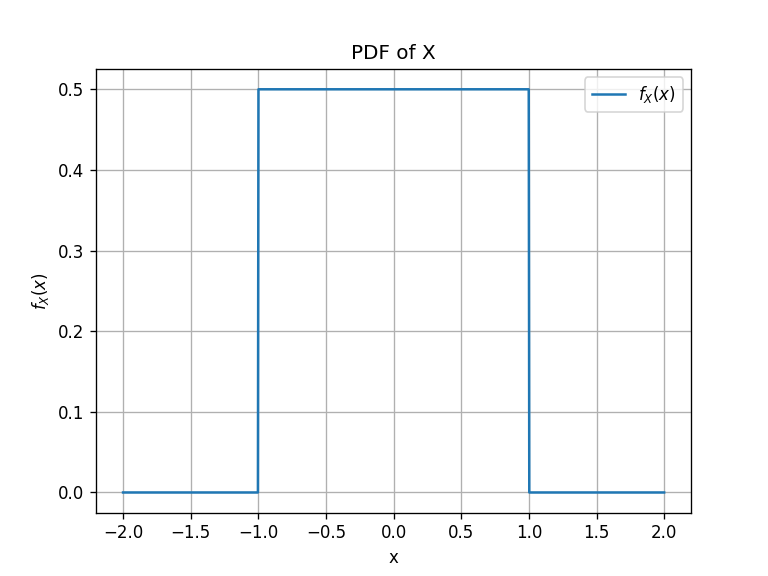
\includegraphics[width=0.5\textwidth]{3.png}\label{fig:f4}}
  \hfill
  \subfloat[CDF for Uniform Distribution of X.]{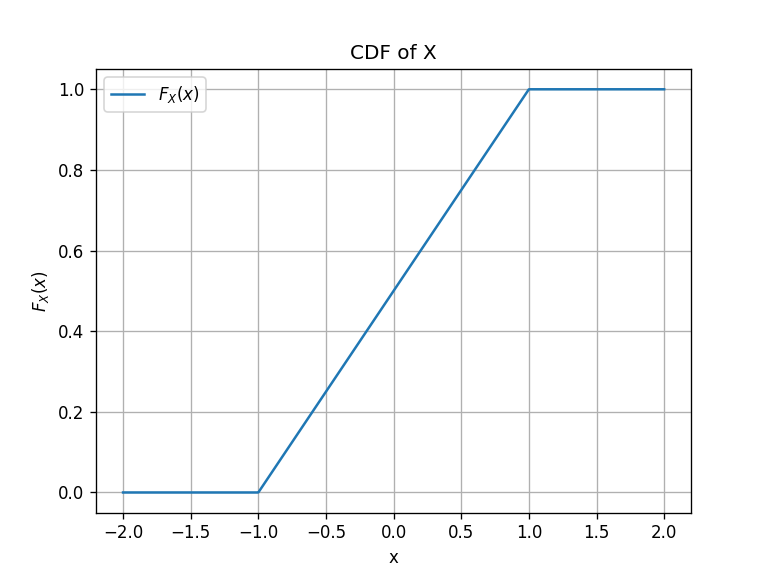
\includegraphics[width=0.5\textwidth]{4.png}\label{fig:f5}}
  \caption{Uniform Distribution}
\end{figure}
\end{frame}
\begin{frame}
\begin{figure}[!tbp]
\centering
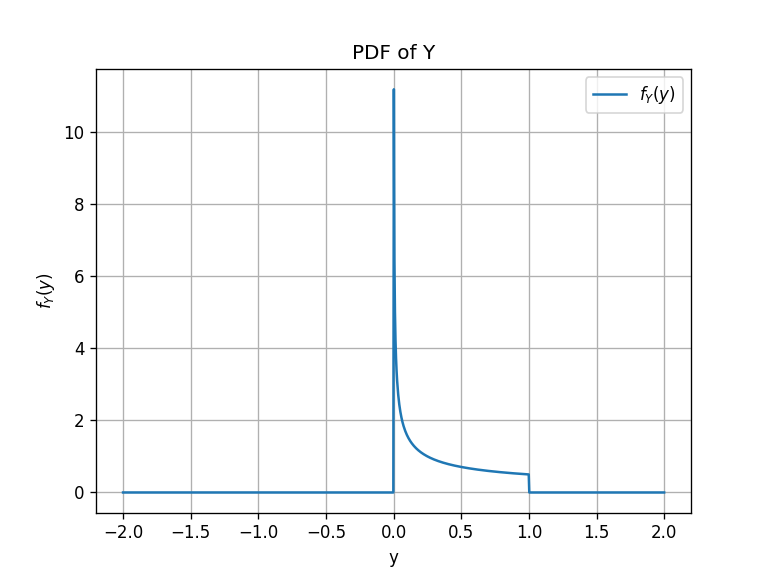
\includegraphics[width=0.5\textwidth]{5.png}
\caption{PDF of Y}
\label{fig:f6}
\end{figure}
\end{frame}
\end{document}